
\part[Recursão]
{Recursão}


\chapter[Recursão]
{Recursão}



\section*{Resumo}

Recursão é uma sub-rotina que pode invocar a si mesma, contendo, a cada chamada, uma pedaço menor da solução final.

%\begin{chapreferences}{1.}
%\bibliography{playcb}
%\bibliographystyle{plain}
%\nocite{cbook}
%\nocite{sb6}
%\nocite{glfw}
%\nocite{cppbook}

%\end{chapreferences}

% \begin{chapreferences}{1}

% \bibitem{sb6}
% {\em OpenGL SuperBible}.
% \newblock Pearson Education Inc, 6 edition, 2014.

% \bibitem{glfw}
% Marcus Geelnard and Camilla Berglund.
% \newblock {\em GLFW - Reference guide}, 2010.
% \newblock API version 2.7.

% \bibitem{cbook}
% Brian~W. Kernighan and Dennis~M. Ritchie.
% \newblock {\em The C Programming Language}.
% \newblock 1989.

% \bibitem{cppbook}
% Stanley~B. Lippman, Josés Lajoile, and Barbara Moo.
% \newblock {\em C++ Primer}.
% \newblock 2013.
% \end{chapreferences}

\section*{Problemas}
\begin{enumerate}

\item
  Construa uma árvore binária recursiva onde o usuário oferece altura, profundidade e ângulo entre ramos. A árvore deverá ser construída tanto para o lado esquerdo, com ângulo entre os galhos de $\theta$ fornecida pelo usuário, quanto para o lado direito, com ângulo $-\theta$.
  \label{ex:cap04_ex2}

  \begin{figure}[H]
    \centerline{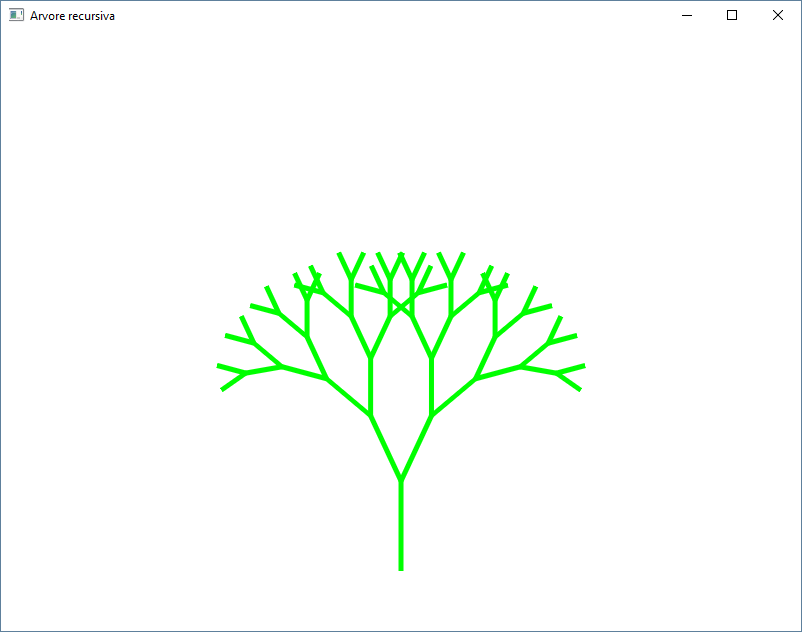
\includegraphics[width=.5\textwidth]{img/cap4_ex17.png}}
    \caption{Árvore Binária com altura $30$, ângulo $25º$ e profundidade $6$}
    \label{fig:cap04_ex2}
  \end{figure}

\item
  Torre de Hanói é um jogo matemático onde seu objetivo é passar os discos de uma torre $A$ para uma torre $B$, utilizando uma torre $C$ como auxiliar. Ele segue as seguintes regras:
  \begin{enumerate}
    \item Só pode mover um disco de cada vez
    \item Só pode mover o disco que estiver mais acima de uma torre e deve-se colocar no topo de outra torre
    \item Não é permitido colocar um disco de tamanho maior em cima de um disco de tamanho menor
  \end{enumerate}

  Ilustre a resolução da torre de Hanói para uma quantidade de 5 discos ou menos.
  \label{ex:cap04_ex1}

  \begin{figure}[H]
    \centerline{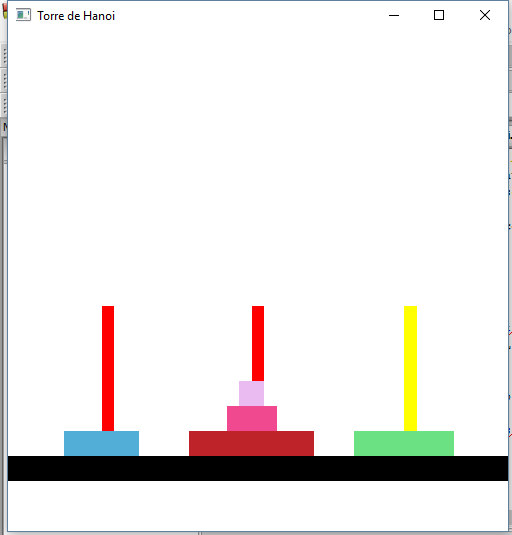
\includegraphics[width=.5\textwidth]{img/cap4_ex13.png}}
    \caption{Solucionador da torre de Hanói}
    \label{fig:cap04_ex1}
  \end{figure}

\item
  Sabe-se que a curva de Koch começa sendo construída com um segmento de reta de tamanho $\frac{n}{3}$. Na extremidade deste primeiro segmento, desenha-se outro segmento de reta de tamanho $\frac{n}{3}$, porém com uma curvatura de $60º$ em relação ao primeiro. Na extremidade deste segundo segmento, desenha-se outra curva de reta de tamanho $\frac{n}{3}$, mas agora com a curvatura de $120º$ em relação ao primeiro. Por fim, desenha-se outro segmento de reta de tamanho $\frac{n}{3}$ na extremidade do terceiro segmento, sem diferença de curvatura.

    \begin{enumerate}
      \item Exiba a curva de Koch de ordem $i$ com tamanho $n$ igual à $180$ unidades centrada na posição $(-100, 0)$. 
        
        (NOTA: a partir de um certo nível de recursão, é possível que a divisão dos segmentos de retas comecem a dividir pixels, tornando inviável a visualização)

      Como sugestão, a Listagem \ref{func:koch} exemplifica um cabeçalho da função \emph{koch}, onde seu primeiro argumento é o ponto de origem, seu segundo argumento é o tamanho do segmento de reta, seu terceiro argumento é a inclinação do segmento e seu quarto argumento é a variável que controla a profundidade de recursão, a qual impede que entre em loop infinito. A função retorna o segundo ponto da reta naquele nível de recursão que deverá ser criada.

      \begin{lstlisting}[caption=Header da função koch, label={func:koch}, language=C++]
      Ponto koch (Ponto from, double len, double theta, int order)
      \end{lstlisting}

        \label{ex:cap04_ex3a}

          \begin{figure*}[!htp]
          \centering
          \begin{subfigure}[b]{0.4\textwidth}
              \centerline{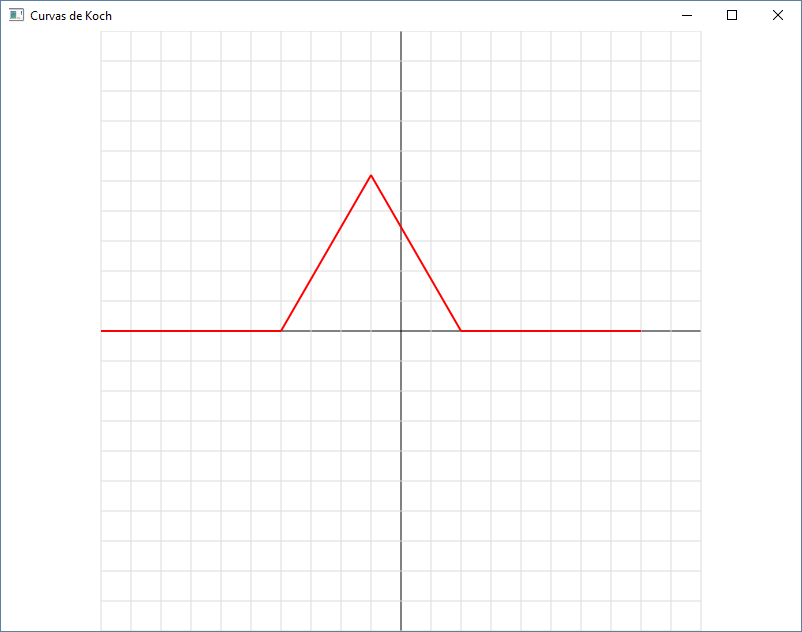
\includegraphics[width=.9\textwidth]{img/cap4_ex14}}
              \caption{Curva de Koch de ordem $1$}
              \label{fig:cap03_ex14a}
          \end{subfigure}
          \hfill
          \begin{subfigure}[b]{0.4\textwidth}
              \centerline{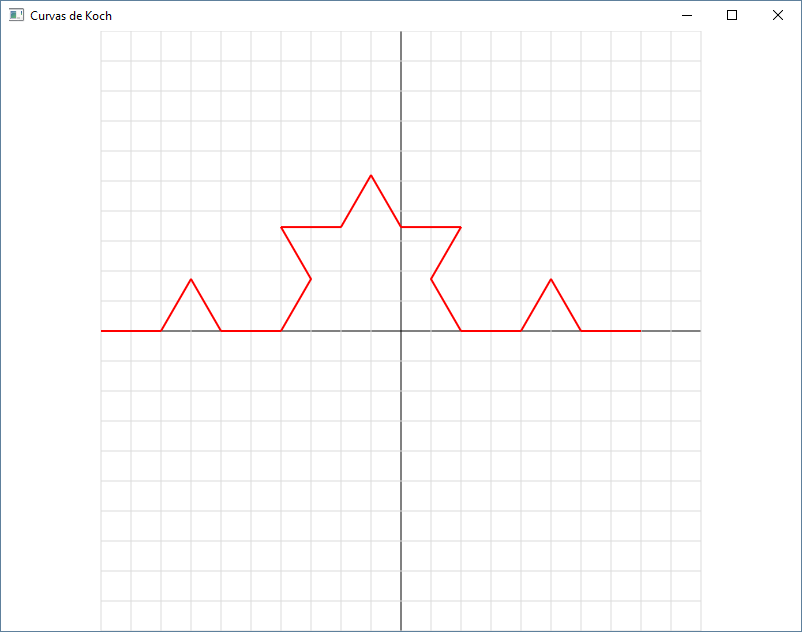
\includegraphics[width=.9\textwidth]{img/cap4_ex14b}}
              \caption{Curva de Koch de ordem $2$}
              \label{fig:cap03_ex14b}
          \end{subfigure}
          \hfill
          \begin{subfigure}[b]{0.4\textwidth}
              \centerline{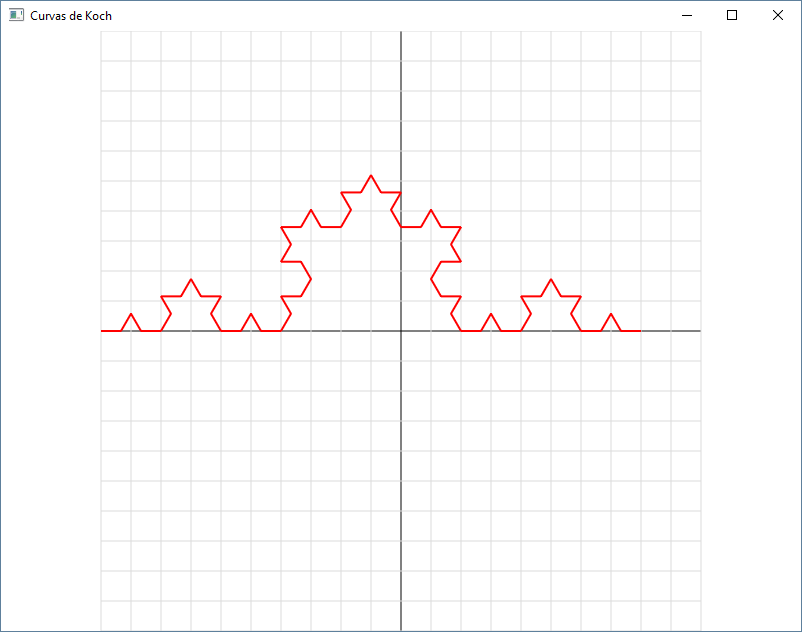
\includegraphics[width=.9\textwidth]{img/cap4_ex14c}}
              \caption{Curva de Koch de ordem $3$}
              \label{fig:cap03_ex14c}
          \end{subfigure}
          \hfill
          \begin{subfigure}[b]{0.4\textwidth}
              \centerline{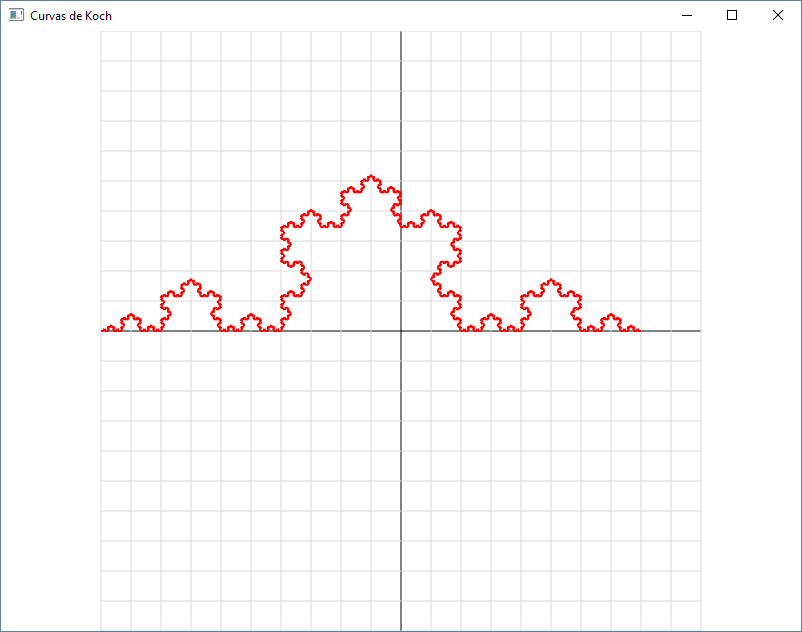
\includegraphics[width=.9\textwidth]{img/cap4_ex14d}}
              \caption{Curva de Koch de ordem $6$}
              \label{fig:cap03_ex14d}
          \end{subfigure}
          
          \caption{
            \label{fig:koch}%
            Curva de Koch
          }

        \end{figure*}

  \label{ex:cap03_ex27}

      \item Utilize a curva de Koch criada no exercício \ref{ex:cap04_ex3a} para criar outras duas curvas, com uma diferença de angulação: a primeira curva será criada da mesma maneira no exercício \ref{ex:cap04_ex3a}; a segunda curva será inclinada em $120º$ e; a terceira curva será inclinada em $-120º$. 

      As Figuras \ref{fig:flocos} ilustram as três retas, onde a primeira curva, com inclinação $0º$, está representada em vermelho, a segunda, com inclinação de $120º$ está representada em verde e a terceira curva, com inclinação $-120º$ está representada em azul.
      \label{ex:cap04_ex3b}

      \begin{figure}[!htp]
          \centering
          \begin{subfigure}[b]{0.4\textwidth}
              \centerline{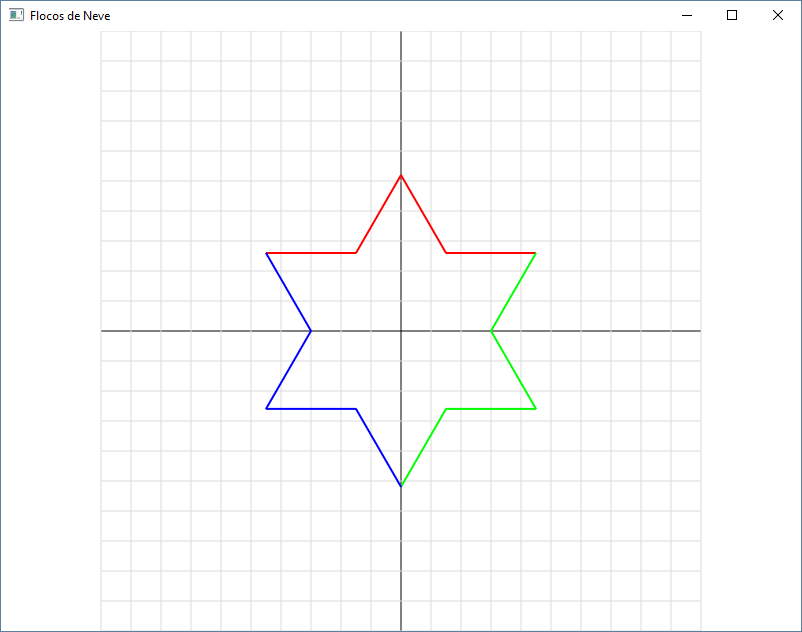
\includegraphics[width=.9\textwidth]{img/cap4_ex15}}
              \caption{Floco de neve de ordem $1$}
              \label{fig:cap04_ex15a}
          \end{subfigure}
          \hfill
          \begin{subfigure}[b]{0.4\textwidth}
              \centerline{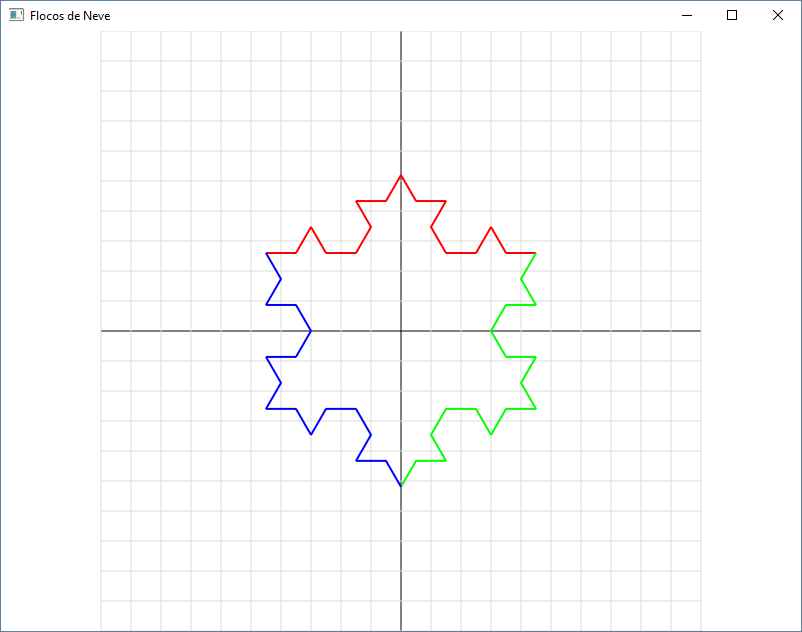
\includegraphics[width=.9\textwidth]{img/cap4_ex15b}}
              \caption{Floco de neve de ordem $2$}
              \label{fig:cap04_ex15b}
          \end{subfigure}
          \hfill
          \begin{subfigure}[b]{0.4\textwidth}
              \centerline{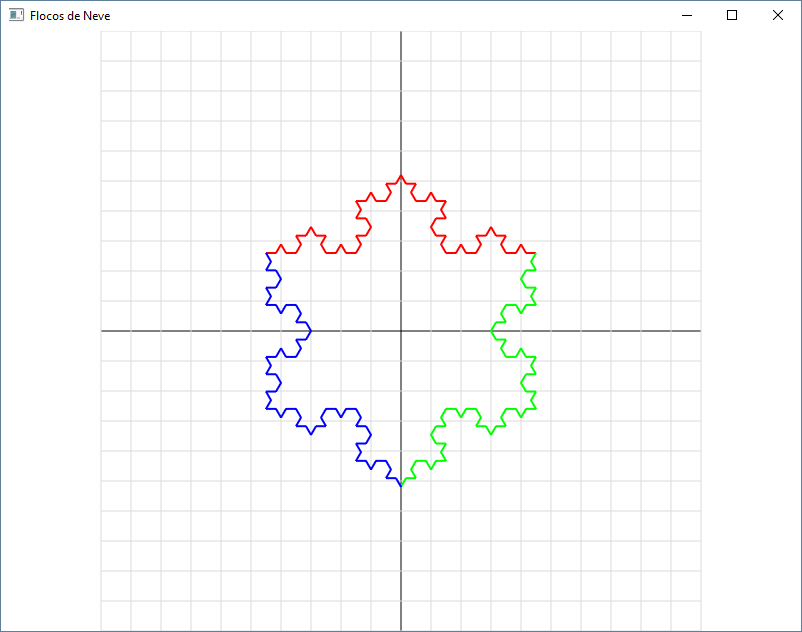
\includegraphics[width=.9\textwidth]{img/cap4_ex15c}}
              \caption{Floco de neve de ordem $3$}
              \label{fig:cap04_ex15c}
          \end{subfigure}
          \hfill
          \begin{subfigure}[b]{0.4\textwidth}
              \centerline{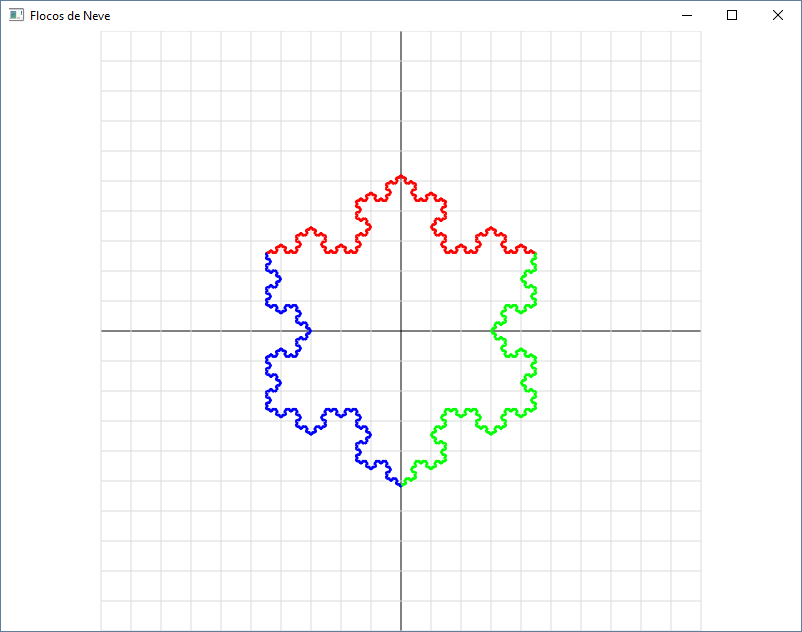
\includegraphics[width=.9\textwidth]{img/cap4_ex15d}}
              \caption{Floco de neve de ordem $6$}
              \label{fig:cap04_ex15d}
          \end{subfigure}

          \caption{
            \label{fig:flocos}%
            Floco de neve
          }

        \end{figure}
    \end{enumerate}

  \label{ex:cap04_ex3}

\item
  A curva de Sierpiński é uma curva do tipo \emph{space-filling curve}, a qual significa que ela tenta ocupar todo espaço disponível sem ser cruzar. Ela pode ser implementada utilizando quatro funções mutuamente recursivas, \emph{A, B, C} e \emph{D}. A Figura \ref{fig:cap04_ex16} ilustra essa curva com as 4 curvas básicas. A curva A está representado em vermelho, a curva B em verde, a curva C em azul e a curva D em amarelo, sendo as curvas que conectam estas 4 curvas básicas representadas em preto.

   \begin{figure}[ht]
    \centerline{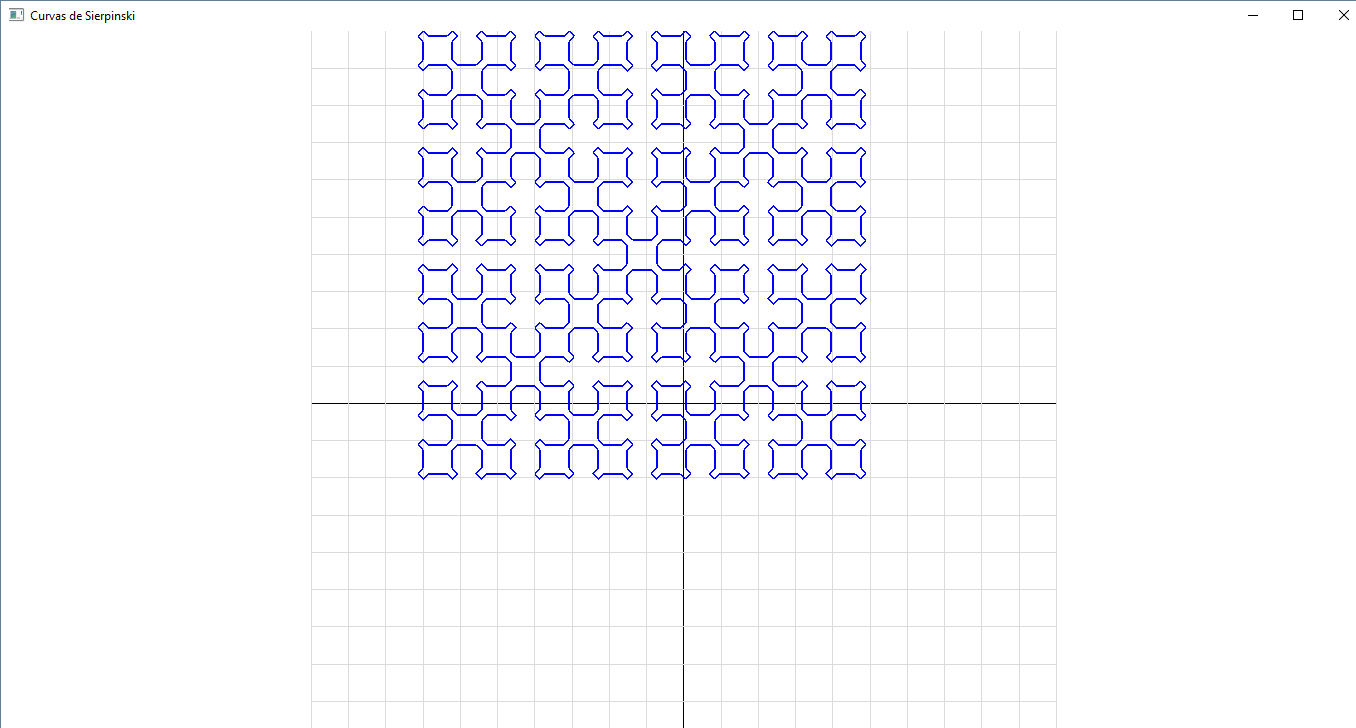
\includegraphics[width=.5\textwidth]{img/cap4_ex16.png}}
    \caption{Curva de Sierpiński de ordem $1$ com ângulo de $45º$}
    \label{fig:cap04_ex16}
  \end{figure}


  \begin{itemize}
    \item
      O programa inicia com uma curva básica \emph{S} dada pelo padrão A 
      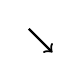
\begin{tikzpicture}
        \draw[thick,->] (0.0,0.30) -- (0.30,0.0);
      \end{tikzpicture}
      , B
      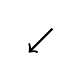
\begin{tikzpicture}
        \draw[thick,->] (0.30,0.30) -- (0.0,0.0);
      \end{tikzpicture}
      , C
      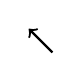
\begin{tikzpicture}
        \draw[thick,->] (0.30,0.0) -- (0.0,0.30);
      \end{tikzpicture}
      e D
      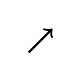
\begin{tikzpicture}
        \draw[thick,->] (0.0,0.0) -- (0.30,0.30);
      \end{tikzpicture}
      . As setam indicam a virada do ângulo que as retas \emph{fecham} os desenhos das funções.
    \item
      A curva A é dada pelo padrão A
      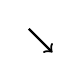
\begin{tikzpicture}
        \draw[thick,->] (0.0,0.30) -- (0.30,0.0);
      \end{tikzpicture}
      , B
      \begin{tikzpicture}
        \draw[thick,->] (0.0,0.0) -- (0.30,0.0);
      \end{tikzpicture}
      , D
      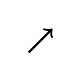
\begin{tikzpicture}
        \draw[thick,->] (0.0,0.0) -- (0.30,0.30);
      \end{tikzpicture}
      A
    \item
      A curva B é dada pelo padrão B
      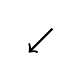
\begin{tikzpicture}
        \draw[thick,->] (0.30,0.30) -- (0.0,0.0);
      \end{tikzpicture}
      , C
      \begin{tikzpicture}
        \draw[thick,->] (0.30,0.30) -- (0.30,0.0);
      \end{tikzpicture}
      , A
      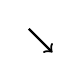
\begin{tikzpicture}
        \draw[thick,->] (0.0,0.30) -- (0.30,0.0);
      \end{tikzpicture}
      B
    \item
      A curva C é dada pelo padrão C
      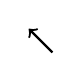
\begin{tikzpicture}
        \draw[thick,->] (0.30,0.0) -- (0.0,0.30);
      \end{tikzpicture}
      , D
      \begin{tikzpicture}
        \draw[thick,->] (0.30,0.0) -- (0.0,0.0);
      \end{tikzpicture}
      , B
      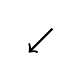
\begin{tikzpicture}
        \draw[thick,->] (0.30,0.30) -- (0.0,0.0);
      \end{tikzpicture}
      C
    \item
      A curva D é dada pelo padrão D
      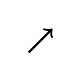
\begin{tikzpicture}
        \draw[thick,->] (0.0,0.0) -- (0.30,0.30);
      \end{tikzpicture}
      , A
      \begin{tikzpicture}
        \draw[thick,->] (0.30,0.0) -- (0.30,0.30);
      \end{tikzpicture}
      , C
      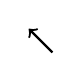
\begin{tikzpicture}
        \draw[thick,->] (0.30,0.0) -- (0.0,0.30);
      \end{tikzpicture}
      D
  \end{itemize}
  Considere o ângulo de inclinação da curva de Sierpiński como $45º$, ou seja, as retas desenhadas tem uma inclinação de $45º$ entre si. Considere também que a curva tenha uma altura $h$ de $40$ unidades e que, caso a ordem de recusão $n$ seja maior que $0$, a altura será determinada por $\frac{h}{n^{2}}$. A criação das curvas se inicia no ponto $p$ em $(-70, 100)$. 

  Considere que a Listagem \ref{func:sier} seja a função que calcula o próximo ponto baseando no ângulo de inclinação e desenha esta reta. Estes fatores são passados de acordo com a Listagem \ref{func:mainsier}.
  \label{ex:cap04_ex4}

  \begin{lstlisting}[caption=Criação da Curva de Sierpiński, label={func:sier}, language=C++]
      Ponto reta(int fator, int h, Ponto p) {
        // ang é para multiplicar por 45 graus
        Ponto p1;
        double ar = fator * 45.0 * PI/180;

        p1.x = p.x + h*cos(ar);
        p1.y = p.y + h*sin(ar);
        CriaReta(p,p1);
        Grafite(2);
        Pintar(0,0,255);
        return p1;
      }
      \end{lstlisting}

    \begin{lstlisting}[caption=Função main Curva de Sierpiński, label={func:mainsier}, language=C++]
      int main() {

        Ponto p;
        int   k; 
        float   h = 40;

        printf("Insira a ordem para a criacao das curvas: ");
        scanf("%d", &k);

        p.x = -70; p.y = 100; //ordem=1 cabe todo na tela


        MostraPlanoCartesiano(10);
        AbreJanela(800,600, "Curvas de Sierpinski");
        PintarFundo(255, 255, 255);


        if (k>0) h /= k*k;
        p = A(k,h, p); 
        p = reta(7,h, p); //calcula o proximo ponto onde a outra reta deve comecar

        p = B(k,h, p); 
        p = reta(5,h, p); 

        p = C(k,h, p); 
        p = reta(3,h, p);

        p = D(k,h, p); 
        p = reta(1,h, p);

        Desenha();

        return 0;
      }
      \end{lstlisting}

  Implemente as funções $A$, $B$, $C$ e $D$ da curva de Sierpiński.

  \begin{figure*}[!htp]
          \centering
          \begin{subfigure}[b]{0.4\textwidth}
              \centerline{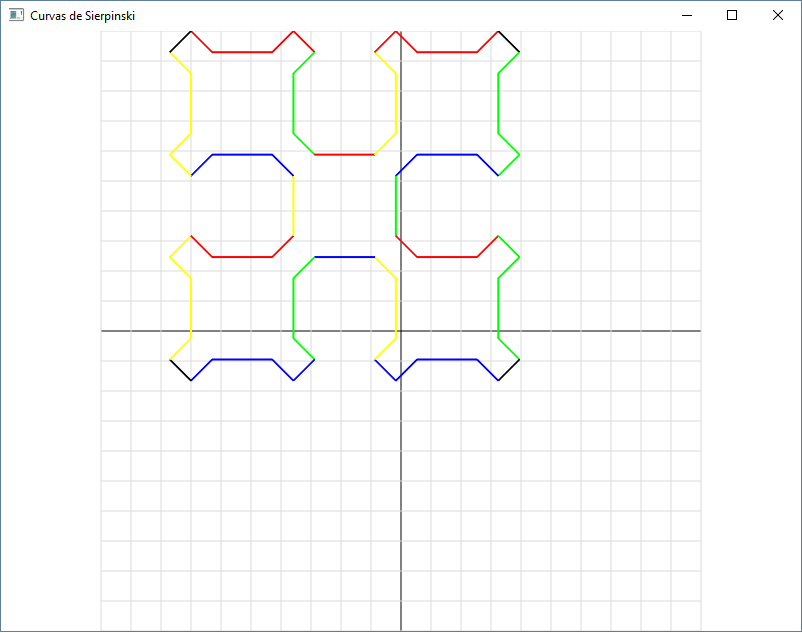
\includegraphics[width=.9\textwidth]{img/cap4_ex16b}}
              \caption{Curva de Sierpiński de ordem $2$}
              \label{fig:cap03_ex14a}
          \end{subfigure}
          \hfill
          \begin{subfigure}[b]{0.4\textwidth}
              \centerline{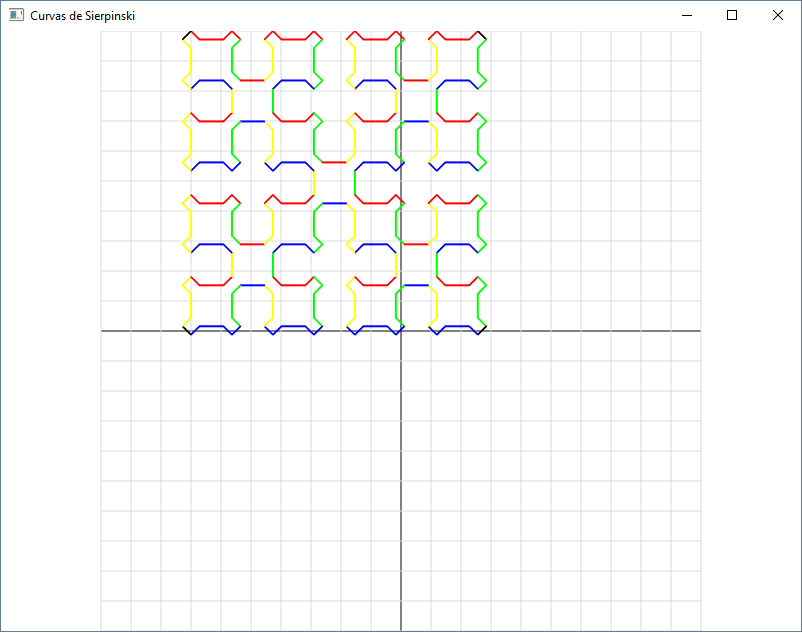
\includegraphics[width=.9\textwidth]{img/cap4_ex16c}}
              \caption{Curva de Sierpiński de ordem $3$}
              \label{fig:cap03_ex14b}
          \end{subfigure}
          
          \caption{
            \label{fig:koch}%
            Curva de Sierpiński
          }

        \end{figure*}
  
\end{enumerate}

\section*{Soluções}

\subsection*{Exercício \ref{ex:cap04_ex2} }

Esta prática reforça que os valores da estrutura \emph{Ponto} podem ser ponto flutuantes.
\lstinputlisting[caption=Árvore recursiva, style=customc, label=lst:cap4_ex3]{src/ex17_arvore.cpp}

\subsection*{Exercício \ref{ex:cap04_ex1} }

Esta prática ilustra como mover cada geometria utilizando retorno da função \emph{CriaGrupo} para mover cada peça da torre de Hanoi para uma posição específica.
\lstinputlisting[caption=Código fonte da torre de Hanói, style=customc, label=lst:cap4_ex1]{src/ex13_hanoi.cpp}

\subsection*{Exercício \ref{ex:cap04_ex3} }
\subsubsection*{Item \ref{ex:cap04_ex3a}}

Esta prática reforça o modo de utilização da função CriaReta, usando a função \emph{movaCaneta}, na linha \ref{line:movaCaneta}.
\lstinputlisting[caption=Código fonte da curva de koch, style=customc, label=lst:cap4_ex2a]{src/ex14_koch.cpp}

\subsubsection*{Item \ref{ex:cap04_ex3b}}
Esta prática é uma evolução do exercício \ref{ex:cap04_ex3a}.
\lstinputlisting[caption=Código fonte do floco de neve, style=customc, label=lst:cap4_ex2b]{src/ex15_snowflake.cpp}


\subsection*{Exercício \ref{ex:cap04_ex4} }

Esta prática reforça o modo de utilizar a função \emph{CriaReta}, usando as implementações das funções das linhas \ref{line:pontoA}, \ref{line:pontoB}, \ref{line:pontoC} e \ref{line:pontoD}. Além disso, exercita fundamentalmente recursões mútuas entre 4 funções.
\lstinputlisting[caption=Código fonte da curva de Sierpiński, style=customc, label=lst:cap4_ex1]{src/ex16_sierpinski.cpp}